\documentclass[12pt]{article}
\setlength{\oddsidemargin}{0in}
\setlength{\evensidemargin}{0in}
\setlength{\textwidth}{6.5in}
\setlength{\parindent}{0in}
\setlength{\parskip}{\baselineskip}

\usepackage[letterpaper, portrait, margin=1in]{geometry}
\usepackage[usenames, dvipsnames, rgb]{xcolor}
\usepackage{amsmath,amsfonts,amssymb,circuitikz,pdfpages,tikz,fancyvrb}

\usetikzlibrary{matrix,calc,circuits.logic.US, shapes.geometric}
\tikzstyle{branch}=[fill, shape=circle, minimum size=3pt, inner sep=0pt]

%isolated term
%#1 - Optional. Space between node and grouping line. Default=0
%#2 - node
%#3 - filling color
\newcommand{\implicantsol}[3][0]{
    \draw[rounded corners=3pt, fill=#3, opacity=0.3] ($(#2.north west)+(135:#1)$) rectangle ($(#2.south east)+(-45:#1)$);
    }


%internal group
%#1 - Optional. Space between node and grouping line. Default=0
%#2 - top left node
%#3 - bottom right node
%#4 - filling color
\newcommand{\implicant}[4][0]{
    \draw[rounded corners=3pt, fill=#4, opacity=0.3] ($(#2.north west)+(135:#1)$) rectangle ($(#3.south east)+(-45:#1)$);
    }

%group lateral borders
%#1 - Optional. Space between node and grouping line. Default=0
%#2 - top left node
%#3 - bottom right node
%#4 - filling color
\newcommand{\implicantcostats}[4][0]{
    \draw[rounded corners=3pt, fill=#4, opacity=0.3] ($(rf.east |- #2.north)+(90:#1)$)-| ($(#2.east)+(0:#1)$) |- ($(rf.east |- #3.south)+(-90:#1)$);
    \draw[rounded corners=3pt, fill=#4, opacity=0.3] ($(cf.west |- #2.north)+(90:#1)$) -| ($(#3.west)+(180:#1)$) |- ($(cf.west |- #3.south)+(-90:#1)$);
}

%group top-bottom borders
%#1 - Optional. Space between node and grouping line. Default=0
%#2 - top left node
%#3 - bottom right node
%#4 - filling color
\newcommand{\implicantdaltbaix}[4][0]{
    \draw[rounded corners=3pt, fill=#4, opacity=0.3] ($(cf.south -| #2.west)+(180:#1)$) |- ($(#2.south)+(-90:#1)$) -| ($(cf.south -| #3.east)+(0:#1)$);
    \draw[rounded corners=3pt, fill=#4, opacity=0.3] ($(rf.north -| #2.west)+(180:#1)$) |- ($(#3.north)+(90:#1)$) -| ($(rf.north -| #3.east)+(0:#1)$);
}

%group corners
%#1 - Optional. Space between node and grouping line. Default=0
%#2 - filling color
\newcommand{\implicantcantons}[2][0]{
    \draw[rounded corners=3pt, opacity=.3] ($(rf.east |- 0.south)+(-90:#1)$) -| ($(0.east |- cf.south)+(0:#1)$);
    \draw[rounded corners=3pt, opacity=.3] ($(rf.east |- 8.north)+(90:#1)$) -| ($(8.east |- rf.north)+(0:#1)$);
    \draw[rounded corners=3pt, opacity=.3] ($(cf.west |- 2.south)+(-90:#1)$) -| ($(2.west |- cf.south)+(180:#1)$);
    \draw[rounded corners=3pt, opacity=.3] ($(cf.west |- 10.north)+(90:#1)$) -| ($(10.west |- rf.north)+(180:#1)$);
    \fill[rounded corners=3pt, fill=#2, opacity=.3] ($(rf.east |- 0.south)+(-90:#1)$) -|  ($(0.east |- cf.south)+(0:#1)$) [sharp corners] ($(rf.east |- 0.south)+(-90:#1)$) |-  ($(0.east |- cf.south)+(0:#1)$);
    \fill[rounded corners=3pt, fill=#2, opacity=.3] ($(rf.east |- 8.north)+(90:#1)$) -| ($(8.east |- rf.north)+(0:#1)$) [sharp corners] ($(rf.east |- 8.north)+(90:#1)$) |- ($(8.east |- rf.north)+(0:#1)$);
    \fill[rounded corners=3pt, fill=#2, opacity=.3] ($(cf.west |- 2.south)+(-90:#1)$) -| ($(2.west |- cf.south)+(180:#1)$) [sharp corners] ($(cf.west |- 2.south)+(-90:#1)$) |- ($(2.west |- cf.south)+(180:#1)$);
    \fill[rounded corners=3pt, fill=#2, opacity=.3] ($(cf.west |- 10.north)+(90:#1)$) -| ($(10.west |- rf.north)+(180:#1)$) [sharp corners] ($(cf.west |- 10.north)+(90:#1)$) |- ($(10.west |- rf.north)+(180:#1)$);
}

%Empty Karnaugh map 4x4
\newenvironment{Karnaugh}%
{
\begin{tikzpicture}[baseline=(current bounding box.north),scale=0.8]
\draw (0,0) grid (4,4);
\draw (0,4) -- node [pos=1,above right,anchor=south west] {$x_3x_4$} node [pos=0.7,below left,anchor=north east] {$x_1x_2$} ++(135:1);
%
\matrix (mapa) [matrix of nodes,
        column sep={0.8cm,between origins},
        row sep={0.8cm,between origins},
        every node/.style={minimum size=0.3mm},
        anchor=8.center,
        ampersand replacement=\&] at (0.5,0.5)
{
                       \& |(c00)| 00         \& |(c01)| 01         \& |(c11)| 11         \& |(c10)| 10         \& |(cf)| \phantom{00} \\
|(r00)| 00             \& |(0)|  \phantom{0} \& |(1)|  \phantom{0} \& |(3)|  \phantom{0} \& |(2)|  \phantom{0} \&                     \\
|(r01)| 01             \& |(4)|  \phantom{0} \& |(5)|  \phantom{0} \& |(7)|  \phantom{0} \& |(6)|  \phantom{0} \&                     \\
|(r11)| 11             \& |(12)| \phantom{0} \& |(13)| \phantom{0} \& |(15)| \phantom{0} \& |(14)| \phantom{0} \&                     \\
|(r10)| 10             \& |(8)|  \phantom{0} \& |(9)|  \phantom{0} \& |(11)| \phantom{0} \& |(10)| \phantom{0} \&                     \\
|(rf) | \phantom{00}   \&                    \&                    \&                    \&                    \&                     \\
};
}%
{
\end{tikzpicture}
}

%Empty Karnaugh map 4x4
\newenvironment{Karnaugh5}%
{
\begin{tikzpicture}[baseline=(current bounding box.north),scale=0.8]
\draw (0,0) grid (4,4);
\draw (0,4) -- node [pos=1,above right,anchor=south west] {$x_4x_5$} node [pos=0.7,below left,anchor=north east] {$x_2x_3$} ++(135:1);
%
\matrix (mapa) [matrix of nodes,
        column sep={0.8cm,between origins},
        row sep={0.8cm,between origins},
        every node/.style={minimum size=0.3mm},
        anchor=8.center,
        ampersand replacement=\&] at (0.5,0.5)
{
                       \& |(c00)| 00         \& |(c01)| 01         \& |(c11)| 11         \& |(c10)| 10         \& |(cf)| \phantom{00} \\
|(r00)| 00             \& |(0)|  \phantom{0} \& |(1)|  \phantom{0} \& |(3)|  \phantom{0} \& |(2)|  \phantom{0} \&                     \\
|(r01)| 01             \& |(4)|  \phantom{0} \& |(5)|  \phantom{0} \& |(7)|  \phantom{0} \& |(6)|  \phantom{0} \&                     \\
|(r11)| 11             \& |(12)| \phantom{0} \& |(13)| \phantom{0} \& |(15)| \phantom{0} \& |(14)| \phantom{0} \&                     \\
|(r10)| 10             \& |(8)|  \phantom{0} \& |(9)|  \phantom{0} \& |(11)| \phantom{0} \& |(10)| \phantom{0} \&                     \\
|(rf) | \phantom{00}   \&                    \&                    \&                    \&                    \&                     \\
};
}%
{
\end{tikzpicture}
}

%Empty Karnaugh map 2x4
\newenvironment{Karnaughvuit}%
{
\begin{tikzpicture}[baseline=(current bounding box.north),scale=0.8]
\draw (0,0) grid (4,2);
\draw (0,2) -- node [pos=1,above right,anchor=south west] {$x_2x_3$} node [pos=0.7,below left,anchor=north east] {$x_1$} ++(135:1);
%
\matrix (mapa) [matrix of nodes,
        column sep={0.8cm,between origins},
        row sep={0.8cm,between origins},
        every node/.style={minimum size=0.3mm},
        anchor=4.center,
        ampersand replacement=\&] at (0.5,0.5)
{
                      \& |(c00)| 00         \& |(c01)| 01         \& |(c11)| 11         \& |(c10)| 10         \& |(cf)| \phantom{00} \\
|(r00)| 0             \& |(0)|  \phantom{0} \& |(1)|  \phantom{0} \& |(3)|  \phantom{0} \& |(2)|  \phantom{0} \&                     \\
|(r01)| 1             \& |(4)|  \phantom{0} \& |(5)|  \phantom{0} \& |(7)|  \phantom{0} \& |(6)|  \phantom{0} \&                     \\
|(rf) | \phantom{00}  \&                    \&                    \&                    \&                    \&                     \\
};
}%
{
\end{tikzpicture}
}

%Empty Karnaugh map 2x2
\newenvironment{Karnaughquatre}%
{
\begin{tikzpicture}[baseline=(current bounding box.north),scale=0.8]
\draw (0,0) grid (2,2);
\draw (0,2) -- node [pos=0.7,above right,anchor=south west] {b} node [pos=0.7,below left,anchor=north east] {a} ++(135:1);
%
\matrix (mapa) [matrix of nodes,
        column sep={0.8cm,between origins},
        row sep={0.8cm,between origins},
        every node/.style={minimum size=0.3mm},
        anchor=2.center,
        ampersand replacement=\&] at (0.5,0.5)
{
          \& |(c00)| 0          \& |(c01)| 1  \\
|(r00)| 0 \& |(0)|  \phantom{0} \& |(1)|  \phantom{0} \\
|(r01)| 1 \& |(2)|  \phantom{0} \& |(3)|  \phantom{0} \\
};
}%
{
\end{tikzpicture}
}

%Defines 8 or 16 values (0,1,X)
\newcommand{\contingut}[1]{%
\foreach\x[count=\xi from 0]  in {#1}
     \path (\xi) node {\x};
}

%Places 1 in listed positions
\newcommand{\minterms}[1]{%
    \foreach \x in {#1}
        \path (\x) node {1};
}

%Places 0 in listed positions
\newcommand{\maxterms}[1]{%
    \foreach \x in {#1}
        \path (\x) node {0};
}

\newcommand{\overbar}[1]{\mkern 1.5mu\overline{\mkern-1.5mu#1\mkern-1.5mu}\mkern 1.5mu}

\begin{document}
\title{Digital Logic Homework 4}

ECEN 2350 Spring 2017 \hfill Homework 4\\
Samuel Cuthbertson

\hrulefill

  \begin{enumerate}
    \vspace{-4mm}
	   \item \textit{Book Problems: 4.3, 4.21}
     \begin{enumerate}
	      \item[(4.3)] \textit{Consider $f = \overbar{w_1}\overbar{w_3} + w_2\overbar{w_3} + \overbar{w_1}w_2$. Use the truth table to derive a circuit for f that uses a 2-to-1 multiplexer.} \\
          Note that the truth table for the above can be found as:
          \begin{center}
            \begin{tabular}{ccc|c}
              $w_1$ & $w_2$ & $w_3$ & f \\
              \hline
              0 & 0 & 0 & 1 \\
              0 & 0 & 1 & 0 \\
              0 & 1 & 0 & 1 \\
              0 & 1 & 1 & 1 \\
              1 & 0 & 0 & 0 \\
              1 & 0 & 1 & 0 \\
              1 & 1 & 0 & 1 \\
              1 & 1 & 1 & 0
            \end{tabular}
          \end{center}
          Which is equvilent to the below circuit, using $w_1$ as the select in a muliplexer.
          \begin{center}
            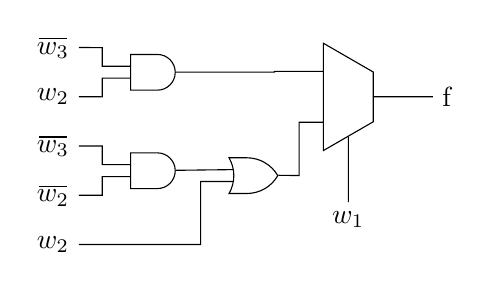
\begin{tikzpicture}[circuit logic US,scale=1.25]
              \node (aaa) at (0, 4.75) {$\overbar{w_3}$};
              \node (aab) at (0, 4.25) {$w_2$};
              \node[and gate US, draw, logic gate inputs=nn] at (1,4.5) (aag) {};
              \draw (aaa)-- ($(aaa) + (0.5,0)$)|- (aag.input 1);
              \draw (aab)-- ($(aab) + (0.5,0)$)|- (aag.input 2);

              \node (aba) at (0, 3.25) {$\overbar{w_2}$};
              \node (abb) at (0, 3.75) {$\overbar{w_3}$};
              \node[and gate US, draw, logic gate inputs=nn] at (1,3.5) (abg) {};
              \draw (aba)-- ($(aba) + (0.5,0)$)|- (abg.input 2);
              \draw (abb)-- ($(abb) + (0.5,0)$)|- (abg.input 1);

              %layer 2
              \node(aca) at (0, 2.75) {$w_2$};
              \node[or gate US, draw, logic gate inputs=nn] at (2,3.45) (bag) {};
              \draw (abg) -- (bag.input 1);
              \draw (aca) -- ($(aca) + (1.5, 0)$)|- (bag.input 2);

              %layer 3
              \node[trapezium, draw, shape border uses incircle, shape border rotate=270, minimum size = 18pt] at (3,4.25) (orf) {};
              \node(ada) at (3, 3) {$w_1$};

              \draw (aag) -- ($(aag) + (1.25,0)$)|- (orf.north west);
              \draw (bag) -- ($(bag) + (0.5,0)$)|- (orf.south west);
              \draw (ada) -- (orf.south);


              %layer 4
              \node (f) at (4,4.25) {f};

              \draw (orf) -- (f);
            \end{tikzpicture}
          \end{center}
        \item[(4.21)] \textit{Write Verilog code for an 8-to-3 binary encoder.}
	        \begin{Verbatim}[fontsize=\small]
module Encode (b, f);
    input [7:0] b;
    output reg [2:0] f;
    always@(*)
    begin
    		case(b)
    		8'b00000001: f = 3'b000;
    		8'b00000010: f = 3'b001;
    		8'b00000100: f = 3'b010;
    		8'b00001000: f = 3'b011;
    		8'b00010000: f = 3'b100;
    		8'b00100000: f = 3'b101;
    		8'b01000000: f = 3'b110;
    		8'b10000000: f = 3'b111;
    		endcase
    end
endmodule

	        \end{Verbatim}
  \end{enumerate}

\newpage
\item \textit{Implement the following circuits using only 2-to-1 mulitplexers.}
  \begin{enumerate}
	   \item $f = \sum m(2,5,6,14)$ \\
	       Note that the truth table, and circuit visually derived from it, are as shown below:
         \begin{center}
	      	  \begin{minipage}{0.2\textwidth}
              \begin{center}
                \begin{tabular}{cccc|c}
                  a & b & c & d & f \\
                  \hline
                  0 & 0 & 0 & 0 & 0 \\
                  0 & 0 & 0 & 1 & 0 \\
                  0 & 0 & 1 & 0 & 1 \\
                  0 & 0 & 1 & 1 & 0 \\
                  0 & 1 & 0 & 0 & 1 \\
                  0 & 1 & 0 & 1 & 0 \\
                  0 & 1 & 1 & 0 & 1 \\
                  0 & 1 & 1 & 1 & 0 \\
                  1 & 0 & 0 & 0 & 0 \\
                  1 & 0 & 0 & 1 & 0 \\
                  1 & 0 & 1 & 0 & 0 \\
                  1 & 0 & 1 & 1 & 0 \\
                  1 & 1 & 0 & 0 & 0 \\
                  1 & 1 & 0 & 1 & 0 \\
                  1 & 1 & 1 & 0 & 1 \\
                  1 & 1 & 1 & 1 & 0
                \end{tabular}
              \end{center}
            \end{minipage}
            \hfill
            \begin{minipage}{0.6\textwidth}
              \begin{center}
                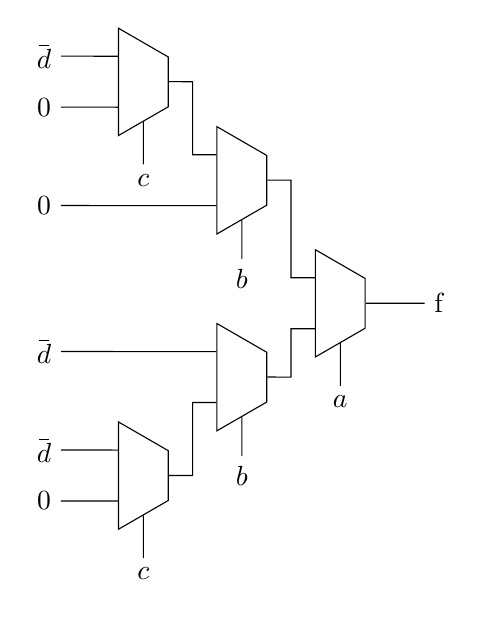
\begin{tikzpicture}[circuit logic US,scale=1.25]
                  \node[trapezium, draw, shape border uses incircle, shape border rotate=270, minimum size = 18pt] at (2,5.5) (bag) {};
                  \node (abc) at (2, 4.5) {$b$};
                  \draw (abc) -- (bag);

                  \node[trapezium, draw, shape border uses incircle, shape border rotate=270, minimum size = 18pt] at (1,6.5) (bcg) {};
                  \node (acb) at (1, 5.5) {$c$};
                  \draw (acb) -- (bcg);

                  \node[trapezium, draw, shape border uses incircle, shape border rotate=270, minimum size = 18pt] at (2,3.5) (cag) {};
                  \node (cbc) at (2, 2.5) {$b$};
                  \draw (cbc) -- (cag);

                  \node[trapezium, draw, shape border uses incircle, shape border rotate=270, minimum size = 18pt] at (1,2.5) (ccg) {};
                  \node (ccb) at (1, 1.5) {$c$};
                  \draw (ccb) -- (ccg);

                  %layer 3
                  \node[trapezium, draw, shape border uses incircle, shape border rotate=270, minimum size = 18pt] at (3,4.25) (orf) {};
                  \node(ada) at (3, 3.25) {$a$};
                  \draw (ada) -- (orf);

                  %layer 2
                  \node (aca) at ($(cag.north west) - (1.75,0)$) {$\overbar{d}$};
                  \draw (aca) -- (cag.north west);
                  \node (afa) at ($(ccg.north west) - (0.75,0)$) {$\overbar{d}$};
                  \draw (afa) -- (ccg.north west);
                  \node (aea) at ($(ccg.south west) - (0.75,0)$) {$0$};
                  \draw (aea) -- (ccg.south west);
                  \draw (bag) -- ($(bag) + (0.5, 0)$) |- (orf.north west);

                  \node (aba) at ($(bag.south west) - (1.75, 0)$) {$0$};
                  \draw (aba) -- (bag.south west);

                  \draw (bcg) -- ($(bcg) + (0.5, 0)$) |- (bag.north west);

                  \draw (cag) -- ($(cag) + (0.5, 0)$) |- (orf.south west);
                  \draw (ccg) -- ($(ccg) + (0.5, 0)$) |- (cag.south west);

                  \node (abb) at ($(bcg.north west) - (0.75, 0)$) {$\overbar{d}$};
                  \draw (abb) -- (bcg.north west);

                  \node (abc) at ($(bcg.south west) - (0.75, 0)$) {$0$};
                  \draw (abc) -- (bcg.south west);

                  %layer 4
                  \node (f) at (4,4.25) {f};

                  \draw (orf) -- (f);
                \end{tikzpicture}
              \end{center}
            \end{minipage}
          \end{center}
	   \item $f = \prod M(3,4,5,6,7)$ \\
     Note that the truth table, and circuit derived from it, are as shown below:
      \begin{center}
        \begin{minipage}{0.2\textwidth}
           \begin{center}
             \begin{tabular}{ccc|c}
               a & b & c & f \\
               \hline
               0 & 0 & 0 & 1 \\
               0 & 0 & 1 & 1 \\
               0 & 1 & 0 & 1 \\
               0 & 1 & 1 & 0 \\
               1 & 0 & 0 & 0 \\
               1 & 0 & 1 & 0 \\
               1 & 1 & 0 & 0 \\
               1 & 1 & 1 & 0 \\
             \end{tabular}
           \end{center}
         \end{minipage}
         \hfill
         \begin{minipage}{0.6\textwidth}
           \begin{center}
             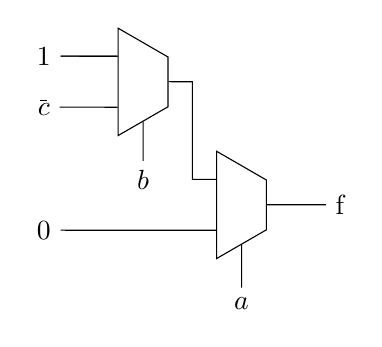
\begin{tikzpicture}[circuit logic US,scale=1.25]
               \node[trapezium, draw, shape border uses incircle, shape border rotate=270, minimum size = 18pt] at (2,5.5) (bag) {};
               \node (abc) at (2, 4.5) {$b$};
               \draw (abc) -- (bag);

               %layer 3
               \node[trapezium, draw, shape border uses incircle, shape border rotate=270, minimum size = 18pt] at (3,4.25) (orf) {};
               \node(ada) at (3, 3.25) {$a$};

               %layer 2
               \node(aca) at ($(orf.south west) - (1.75,0)$) {$0$};
               \draw (aca) -- (orf.south west);
               \draw (bag) -- ($(bag) + (0.5, 0)$) |- (orf.north west);
               \draw (ada) -- (orf.south);

               \node (aba) at ($(bag.south west) - (0.75, 0)$) {$\overbar{c}$};
               \draw (aba) -- (bag.south west);

               \node (abb) at ($(bag.north west) - (0.75, 0)$) {$1$};
               \draw (abb) -- (bag.north west);

               \draw (abb) -- (bag.north west);

               %layer 4
               \node (f) at (4,4.25) {f};

               \draw (orf) -- (f);
             \end{tikzpicture}
           \end{center}
         \end{minipage}
       \end{center}
  \end{enumerate}

\newpage
\item \textit{Convert the following decimal numbers to 32-bit floating point format.}
  \begin{enumerate}
      \item \textit{33554430} \\
          \begin{center}
            First, note that $(\frac{33554430}{2^{24}})_{10} = 1.99...$ and that
            \begin{align*}
              33554430 &= 2^{24} + 2^{23} + 2^{22} + ... + 2^3 + 2^2 \\
              &= (1111 1111 1111 1111 1111 1110)_2 \\
              &= (1.1111 1111 1111 1111 1111 11)_2 * 2^{24} \\
            \end{align*}
            Which implies that $Expontent = 24 \implies E = 24 - 127 = 151 = (10010111)_2$ for the floating point form below.
            \begin{align*}
              &S,E,E,E,E,E,E,E,E,23bitsM \\
              &(0\;10010111\;1111 1111 1111 1111 1111 111)_2
            \end{align*}
          \end{center}
      \item \textit{33554431} \\
      \begin{center}
        First, note that $(\frac{33554431}{2^{24}})_{10} = 1.99...$ and that
        \begin{align*}
          33554430 &= 2^{24} + 2^{23} + 2^{22} + ... + 2^3 + 2^2 + 2^1\\
          &= (1111 1111 1111 1111 1111 1111)_2 \\
          &= (1.1111 1111 1111 1111 1111 111)_2 * 2^{24} \\
        \end{align*}
        Which implies that $Expontent = 24 \implies E = 24 - 127 = 151 = (10010111)_2$ for the floating point form below.
        \begin{align*}
          &S,E,E,E,E,E,E,E,E,23bitsM \\
          &(0\;10010111\;1111 1111 1111 1111 1111 111\color{red}{1}\color{black}{)_2}
        \end{align*}
        However, there needs to be 24 bits in the Mantissa to accurately represent $33554431$. Therefor, there is no way to accuratly represent the given number without double precision or rounding.
      \end{center}
  \end{enumerate}

\vspace{7mm}
\item \textit{Convert the following decimal numbers to fixed point unsigned binary with at least 8-bits of binary precision}
  \begin{enumerate}
      \item \textit{12.45897} \\
          Note that $(12)_{10} = (1100)_2$, and $(.45897)_{10} \approx \frac{1}{4} + \frac{1}{8} + \frac{1}{16} = (.0111)_2$, which implies that $(12.45897)_{10} \approx \boxed{(1100.0111)_2}$
      \item \textit{0.333333} \\
          Note that $.333333 \approx \frac{1}{4} + \frac{1}{16} + \frac{1}{64} +\frac{1}{256} = \boxed{(.01010101)_2}$
  \end{enumerate}

\newpage
\item \textit{For 32-bit Precision wow Floating point numbers, {\tt E=0x00} and {\tt E=0xFF} are used for special numbers (like $0$ and $\infty$). What are the decimal values of the floating point numbers (32-bit) of smallest (non-zero) and largest (non-infinity) magnitude} \\

The smallest number would have {\tt E=0x1} and {\tt M=0x1}, which results in a number of value $(1 + 2^{-24}) * 2^{1-127} \approx \boxed{1.1754945 * 10^{-38}}$ \\

Similarly, the largest number would have {\tt E=0xFE} and {\tt M=b111...111}, which results in $(1 + 2^{-2} + 2^{-4} + .. + 2^{-24}) * 2^{127} \approx \boxed{3.4028235 * 10^{38}}$

\end{enumerate}
\end{document}
